\documentclass[11pt,a4paper,titlepage]{article}
\usepackage[a4paper]{geometry}
\usepackage[utf8]{inputenc}
\usepackage[english]{babel}
\usepackage{lipsum}
\usepackage{eurosym}
\usepackage{rotating}

\usepackage{amsmath, amssymb, amsfonts, amsthm, mathtools}
% mathtools for: Aboxed (put box on last equation in align envirenment)
\usepackage{microtype} %improves the spacing between words and letters

\usepackage{lipsum}
\usepackage{threeparttable}
\usepackage{tabularx}
\usepackage{multirow}
\usepackage{booktabs}
\newcommand{\tabitem}{~~\llap{\textbullet}~~}
\usepackage{graphicx}
\graphicspath{ {./figures/} {./eps/}}
\usepackage{epsfig}
\usepackage{epstopdf}
\usepackage{verbatim}
\usepackage{textcomp}
\usepackage{tikz}
\usetikzlibrary{shapes,arrows}

%%%%%%%%%%%%%%%%%%%%%%%%%%%%%%%%%%%%%%%%%%%%%%%%%%
%% COLOR DEFINITIONS
%%%%%%%%%%%%%%%%%%%%%%%%%%%%%%%%%%%%%%%%%%%%%%%%%%
 % Enabling mixing colors and color's call by 'svgnames'
%%%%%%%%%%%%%%%%%%%%%%%%%%%%%%%%%%%%%%%%%%%%%%%%%%
\definecolor{MyColor1}{HTML}{CC0000} %mix personal color
\newcommand{\textb}{\color{Black} \usefont{OT1}{lmss}{m}{n}}
\newcommand{\blue}{\color{MyColor1} \usefont{OT1}{lmss}{m}{n}}
\newcommand{\blueb}{\color{MyColor1} \usefont{OT1}{lmss}{b}{n}}
\newcommand{\red}{\color{LightCoral} \usefont{OT1}{lmss}{m}{n}}
\newcommand{\green}{\color{Turquoise} \usefont{OT1}{lmss}{m}{n}}
%%%%%%%%%%%%%%%%%%%%%%%%%%%%%%%%%%%%%%%%%%%%%%%%%%


%%%%%%%%%%%%%%%%%%%%%%%%%%%%%%%%%%%%%%%%%%%%%%%%%%
%% FONTS AND COLORS
%%%%%%%%%%%%%%%%%%%%%%%%%%%%%%%%%%%%%%%%%%%%%%%%%%
%    SECTIONS
%%%%%%%%%%%%%%%%%%%%%%%%%%%%%%%%%%%%%%%%%%%%%%%%%%
\usepackage{titlesec}
\usepackage{sectsty}
%%%%%%%%%%%%%%%%%%%%%%%%
%set section/subsections HEADINGS font and color
\sectionfont{\color{MyColor1}}  % sets colour of sections
\subsectionfont{\color{MyColor1}}  % sets colour of sections

%set section enumerator to arabic number (see footnotes markings alternatives)
\renewcommand\thesection{\arabic{section}.} %define sections numbering
\renewcommand\thesubsection{\thesection\arabic{subsection}} %subsec.num.

%define new section style
\newcommand{\mysection}{
\titleformat{\section} [runin] {\usefont{OT1}{lmss}{b}{n}\color{MyColor1}}
{\thesection} {3pt} {} }

%%%%%%%%%%%%%%%%%%%%%%%%%%%%%%%%%%%%%%%%%%%%%%%%%%
%		CAPTIONS
%%%%%%%%%%%%%%%%%%%%%%%%%%%%%%%%%%%%%%%%%%%%%%%%%%
\usepackage{caption}
\usepackage{subcaption}
%%%%%%%%%%%%%%%%%%%%%%%%
\captionsetup[figure]{labelfont={color=MyColor1}}

%%%%%%%%%%%%%%%%%%%%%%%%%%%%%%%%%%%%%%%%%%%%%%%%%%
%		!!!EQUATION (ARRAY) --> USING ALIGN INSTEAD
%%%%%%%%%%%%%%%%%%%%%%%%%%%%%%%%%%%%%%%%%%%%%%%%%%
%using amsmath package to redefine eq. numeration (1.1, 1.2, ...)
%%%%%%%%%%%%%%%%%%%%%%%%
\renewcommand{\theequation}{\thesection\arabic{equation}}

%set box background to grey in align environment
\usepackage{etoolbox}% http://ctan.org/pkg/etoolbox
\makeatletter
\patchcmd{\@Aboxed}{\boxed{#1#2}}{\colorbox{black!15}{$#1#2$}}{}{}%
\patchcmd{\@boxed}{\boxed{#1#2}}{\colorbox{black!15}{$#1#2$}}{}{}%
\makeatother
%%%%%%%%%%%%%%%%%%%%%%%%%%%%%%%%%%%%%%%%%%%%%%%%%%

\newcommand{\DP}[1]{\textcolor{blue}{\textbf{(DP says: #1)}}}
\newcommand{\cri}[1]{\textcolor{green}{\textbf{(Cri says: #1)}}}

\makeatletter
\let\reftagform@=\tagform@
\def\tagform@#1{\maketag@@@{(\ignorespaces\textcolor{red}{#1}\unskip\@@italiccorr)}}
\renewcommand{\eqref}[1]{\textup{\reftagform@{\ref{#1}}}}
\makeatother
\usepackage[hidelinks]{hyperref}

%% LISTS CONFIGURATION %%
\usepackage{enumitem}
\setlist[enumerate,1]{start=0}
\renewcommand{\labelenumii}{\theenumii}
\renewcommand{\theenumii}{\theenumi.\arabic{enumii}.}

\usepackage[acronym]{glossaries}
\newacronym{pmu}{PMU}{Power Management Unit}

%%%%%%%%%%%%%%%%%%%%%%%%%%%%%%%%%%%%%%%%%%%%%%%%%%
%% PREPARE TITLE
%%%%%%%%%%%%%%%%%%%%%%%%%%%%%%%%%%%%%%%%%%%%%%%%%%
\title{\blue User equipment and terminals \\
\blueb With great power comes great responsibility}
\author{Davide Peron\\ Cristina Gava}
\date{\today}
%%%%%%%%%%%%%%%%%%%%%%%%%%%%%%%%%%%%%%%%%%%%%%%%%%

\begin{document}
\maketitle

\tableofcontents
\clearpage

\section{Power Supply} \label{sec:power_supply}

\section{Power Management} \label{sec:power_management}
	\subsection{Wii U}
		The Wii U transformer has a maximum output voltage of 15V and a maximum output current of 5A, so this console consumes $15\cdot 5 = 75W$ while under full load.
		\begin{figure}[ht]
			\centering
			\begin{minipage}{0.45\textwidth}
				\centering
				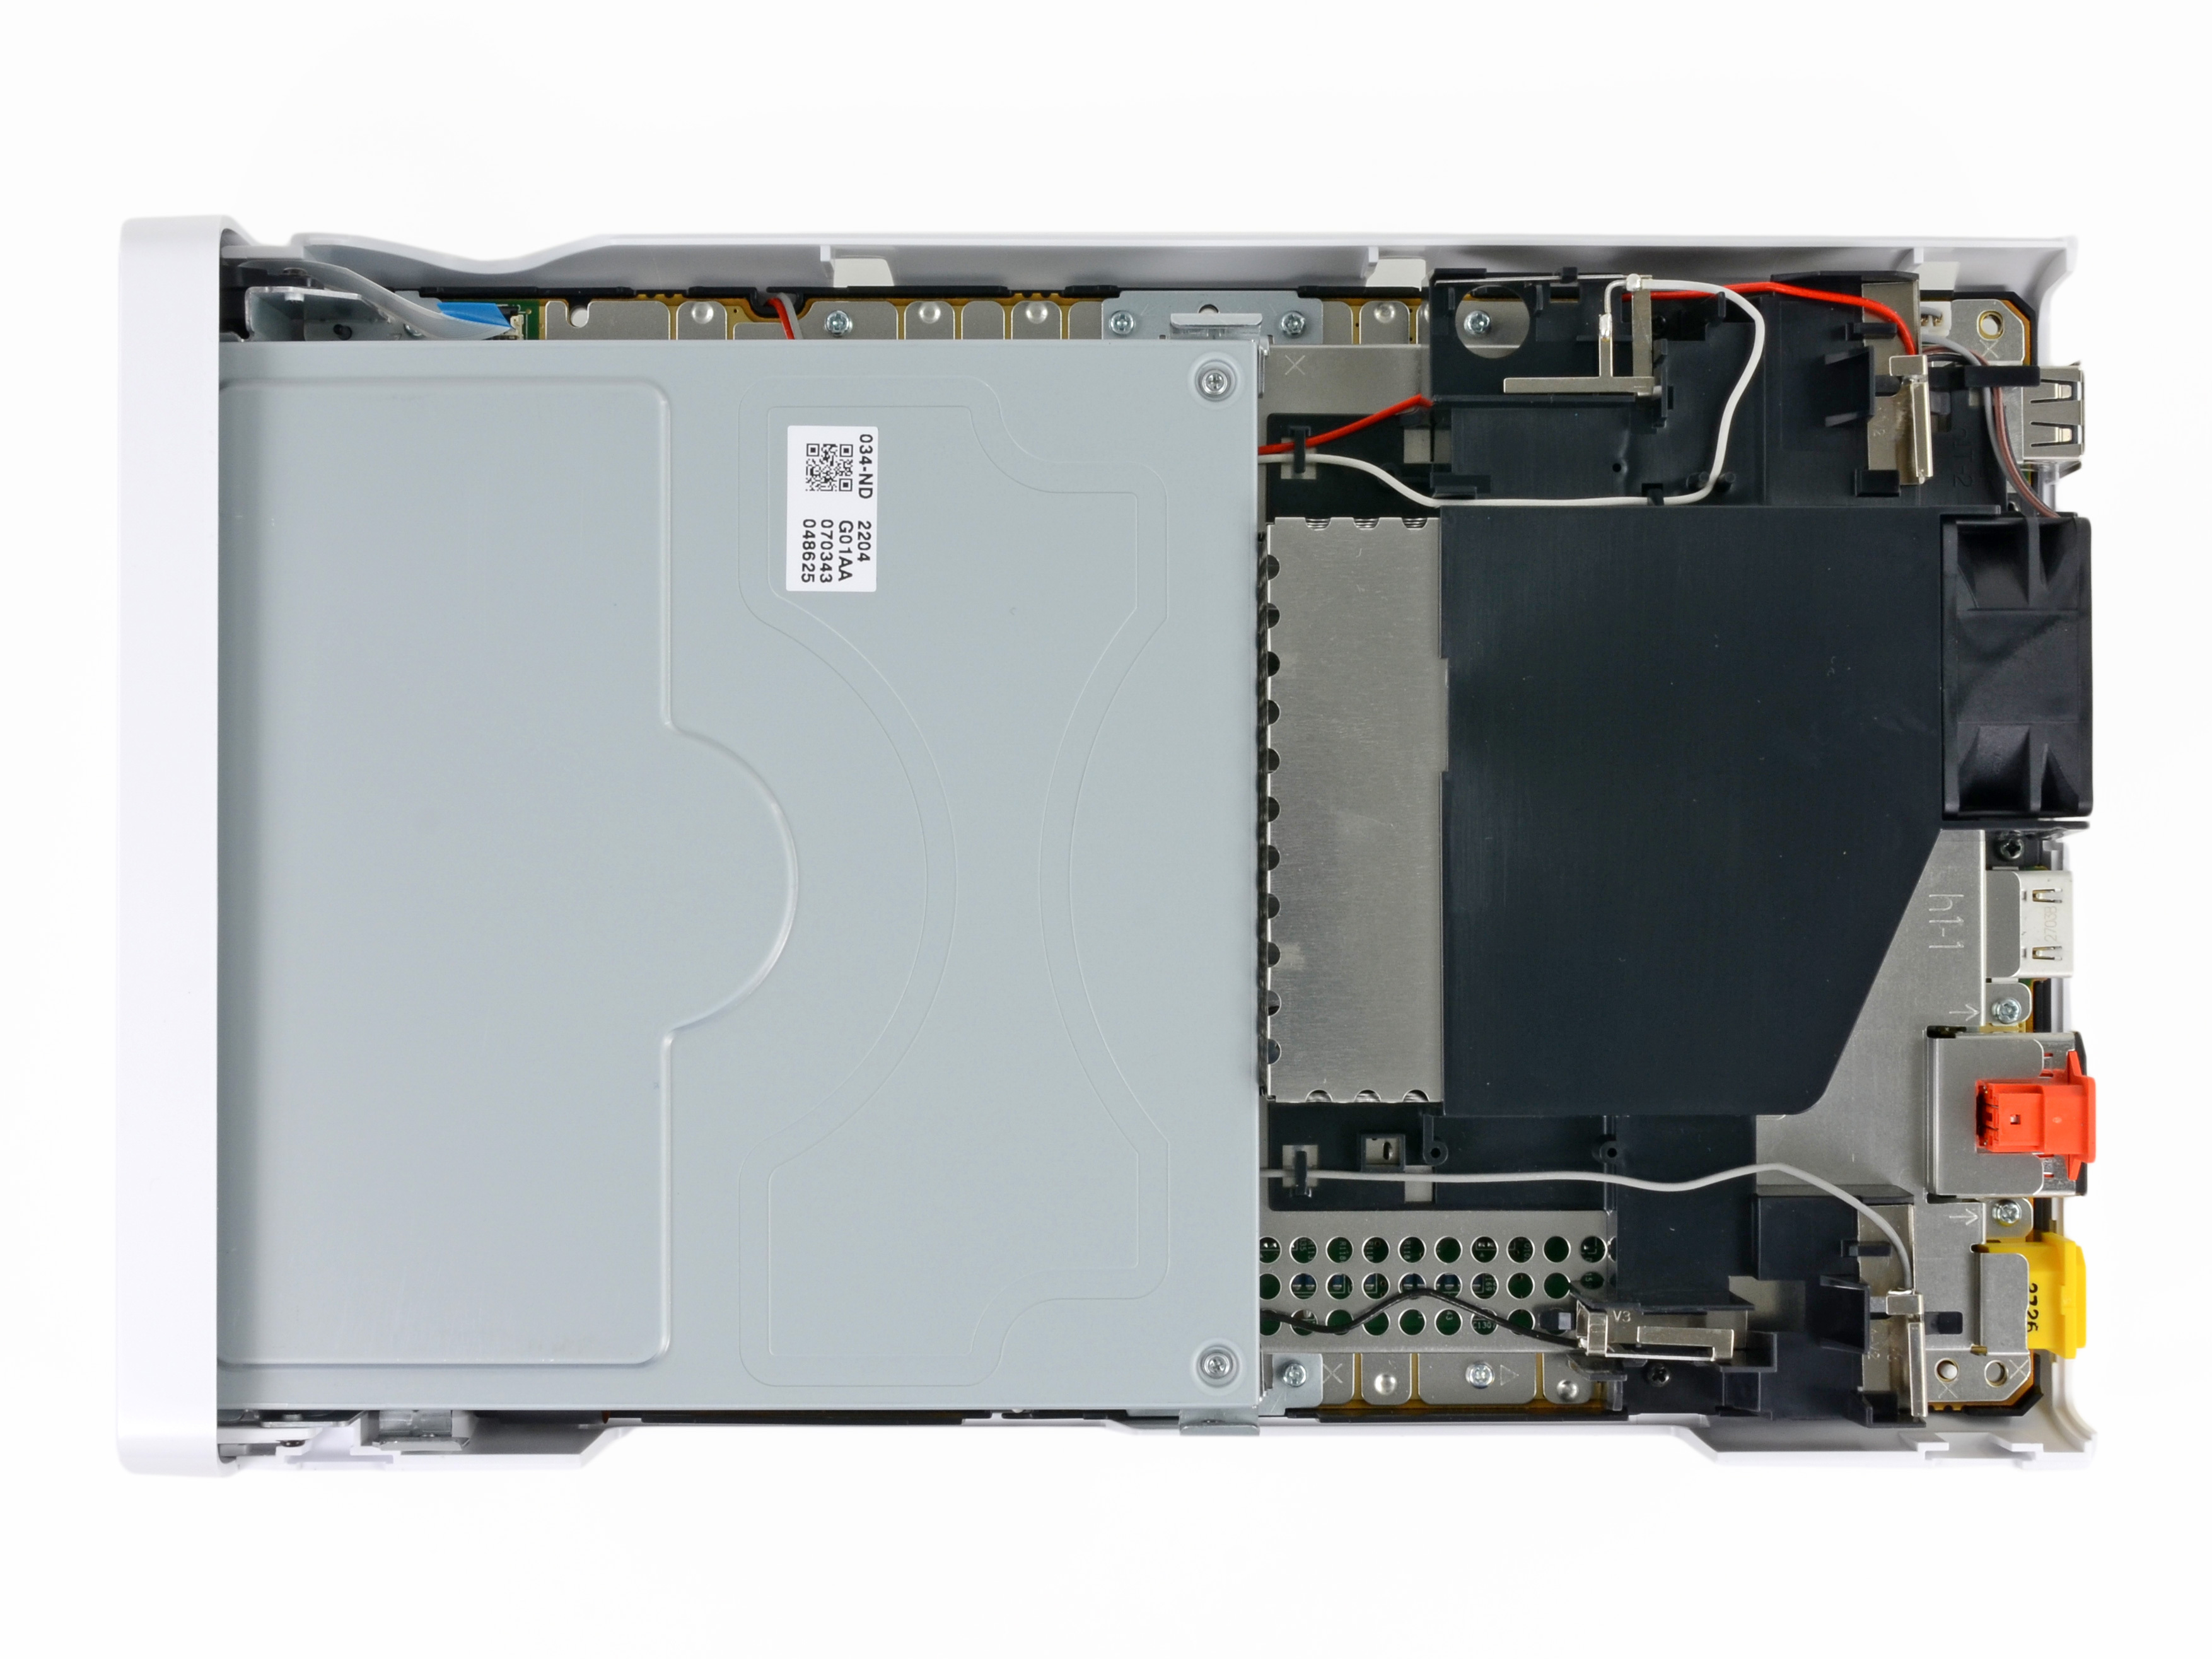
\includegraphics[width=\textwidth]{external_view.jpeg}
				\caption{Wii U without external case}
				\label{fig:external}
			\end{minipage}
			\begin{minipage}{0.45\textwidth}
				\centering
				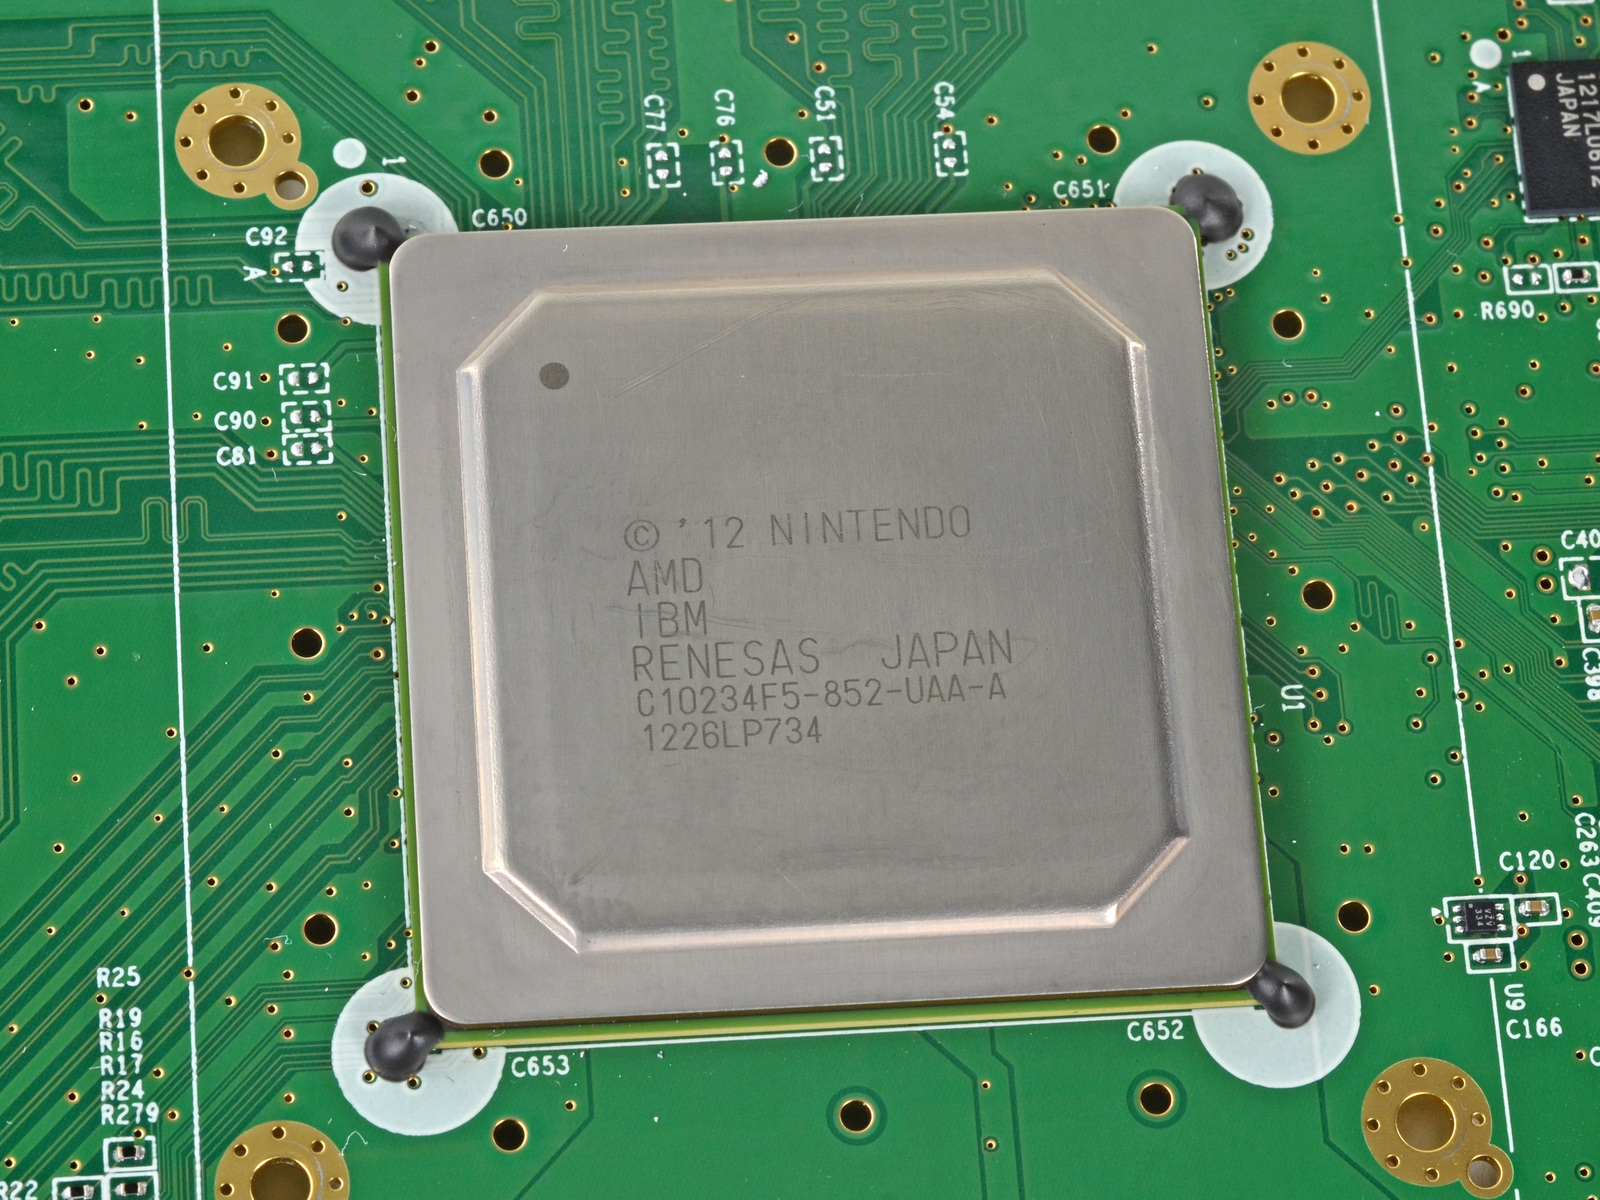
\includegraphics[width=\textwidth]{CPU_&_GPU.png}
				\caption{Wii U Multi Chip Module}
				\label{fig:mcm}
			\end{minipage}
		\end{figure}
		\begin{figure}[ht]
			\centering
			\begin{minipage}{0.45\textwidth}
				\centering
				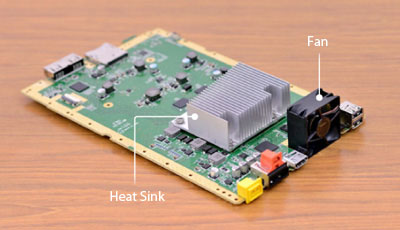
\includegraphics[width=\textwidth]{fan-heatsink.jpeg}
				\caption{Fan and heat sink position}
				\label{fig:fan-heatsink}
			\end{minipage}
			\begin{minipage}{0.45\textwidth}
				\centering
				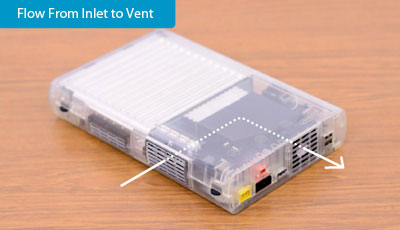
\includegraphics[width=\textwidth]{air_flow.jpeg}
				\caption{Wii U air flow demonstration}
				\label{fig:airflow}
			\end{minipage}
		\end{figure}
		In \autoref{fig:external} is shown the console without its external case.
		The first thing we note is that the bigger components inside the Wii U are the optical drive, a single heat sink used to cool down the entire console and two fans to allow the air to pass through the console.

		Analysing the position of the fan and of the heat sink, we note that the heat sink is over the main source of heat (the CPU and GPU) and it is close to the fan rotated in a way that the air can pass through it, as shown in \autoref{fig:airflow}.

		Removing the heat sink we see another thermal compound that cover both CPU and GPU. These two are put close each other maybe to reduce the latency and power consumption.

	\subsection{GamePad}
		The GamePad transformer has a maximum output voltage of 4.75V and a maximum output current of 1.6A, so this console consumes $4.75\cdot 1.6 = 7.6W$ while under full load.
		\begin{figure}[htbp]
			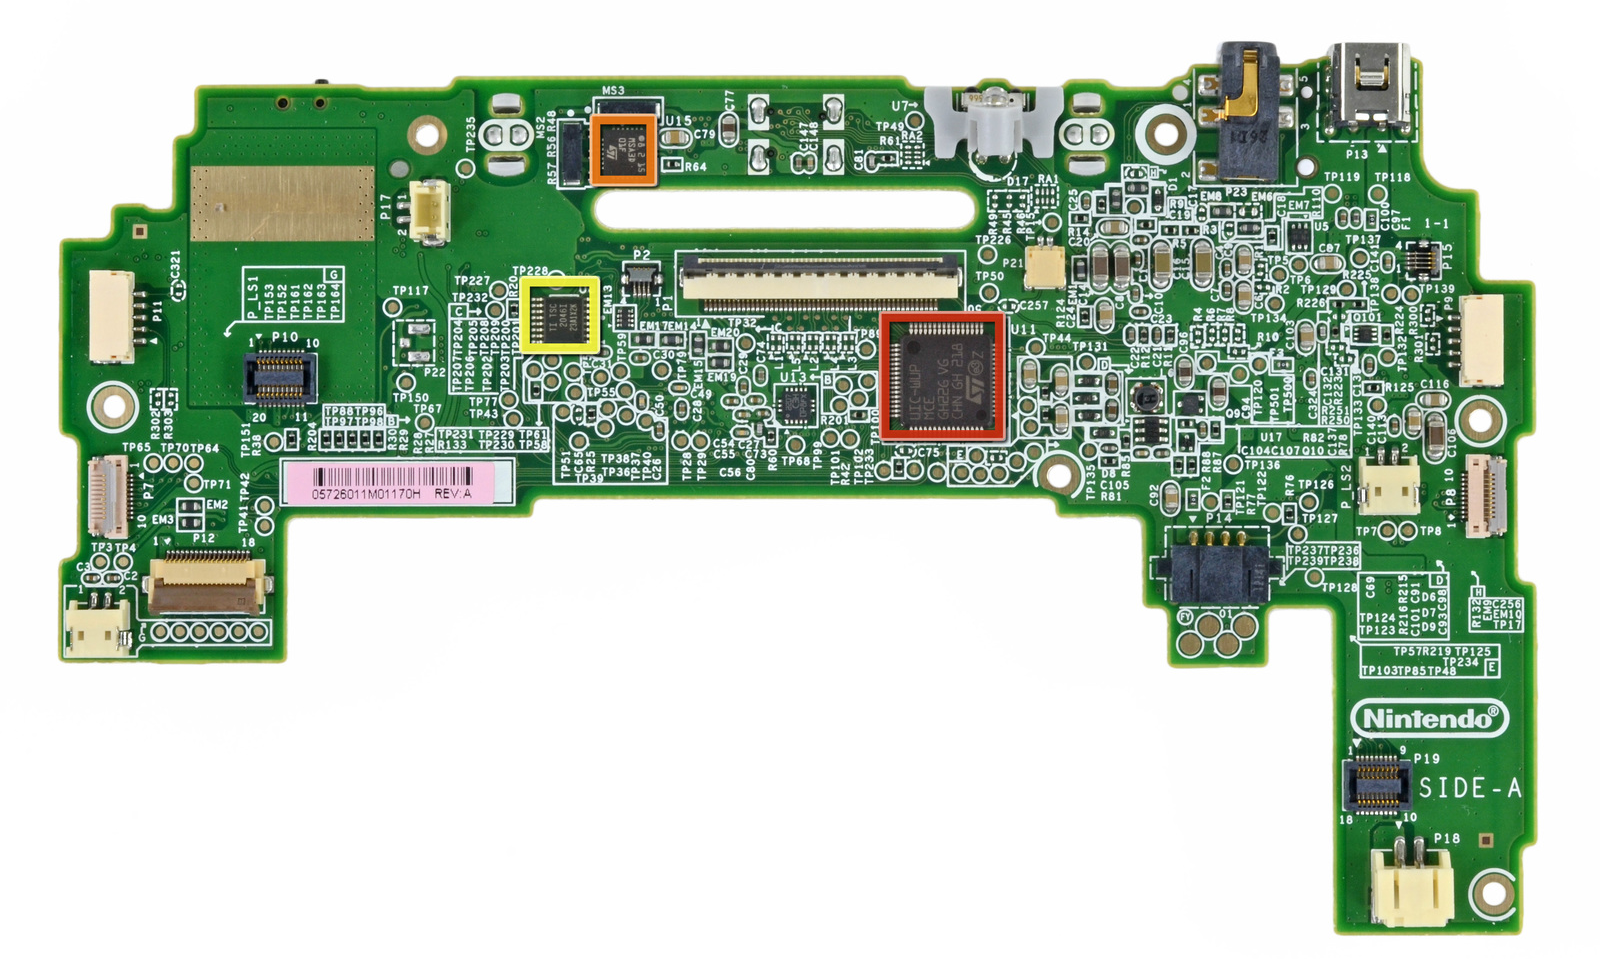
\includegraphics[width=\textwidth]{gamepad_motherboard_front.png}
			\caption{GamePad's motherboard}
			\label{fig:gamepad_motherboard}
		\end{figure}
		\subsubsection{Touch Screen Controller}
			TSC2046I is the touch screen controller used in the GamePad of the Wii U. TSC2046I is a chip integrated in the GamePad's motherboard, specifically is the chip in the yellow square in \autoref{fig:gamepad_motherboard}.

			Checking the datasheet \cite{touchscreen} we can get some interesting information.
			\begin{itemize}
				\item It has an on-chip $2.5V$ voltage reference that can be used for the auxiliary input, battery monitor, and temperature measurement modes. This can be powered down when not used to conserve power.
				\item The power consumption is less than $0.75mW$ at $2.7V$.
			\end{itemize}

			In \autoref{tab:thermal_touch} are summarized the parameters relatively to the thermal management of the chip.

			In \autoref{fig:vref_temp} and \autoref{fig:vref_vcc} is shown as the on-chip reference voltage previously mentioned is actually not fixed at $2.5V$ but is floating around this value and depends on the Temperature and on the input voltage $V_{CC}$. In \autoref{fig:sample_vcc} and \autoref{fig:vcc_temp} is shown as the Sample Rate of the Touch Screen Controller varies with the input voltage and how this last one varies with the temperature.

			In general we can deduct that if $V_{CC}$ is too low (more or less lower than $3V$), both the sample rate and the reference voltage $V_{REF}$ will decrease.


			\begin{table}[htbp]
				\centering
				\begin{tabular}{cc}
				\toprule
				Parameter & Value\\
				\midrule
				Power Dissipation     & 250mW\\
				Maximum Junction Temperature  & $+150^\circ C$\\
				Operating Temperature Range & $-40^\circ C$ to $+85^\circ C$ \\
				Storage Temperature Range & $-65^\circ C$ to $+150^\circ C$ \\
				Lead Temperature  & $+300^\circ C$\\
				\bottomrule
				\end{tabular}
				\caption{Thermal management in TSC2046I}
				\label{tab:thermal_touch}
			\end{table}

			\begin{figure}[htbp]
				\begin{minipage}{.5\textwidth}
					\centering
					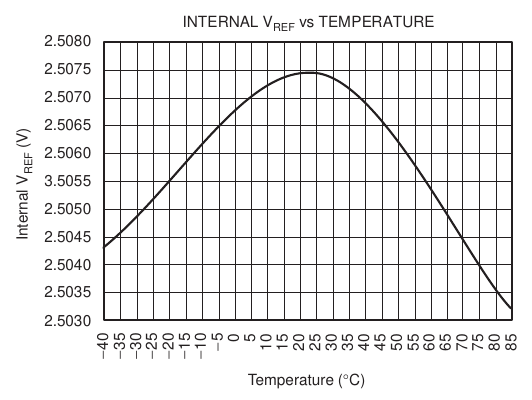
\includegraphics[width=\textwidth]{v_ref_temp.png}
					\caption{Variation of $V_{REF}$ with Temperature}
					\label{fig:vref_temp}
				\end{minipage}
				\begin{minipage}{.5\textwidth}
					\centering
					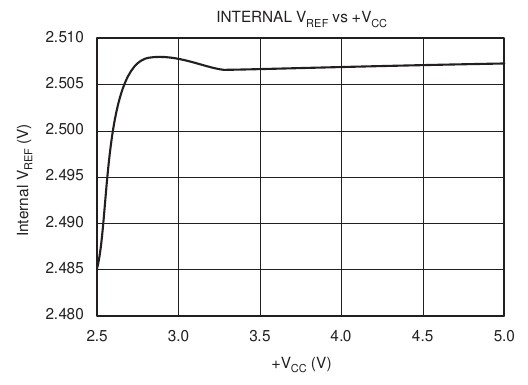
\includegraphics[width=\textwidth]{v_ref_vcc.png}
					\caption{Variation of $V_{REF}$ with $V_{CC}$}
					\label{fig:vref_vcc}
				\end{minipage}
			\end{figure}

			\begin{figure}[htbp]
				\begin{minipage}{.5\textwidth}
					\centering
					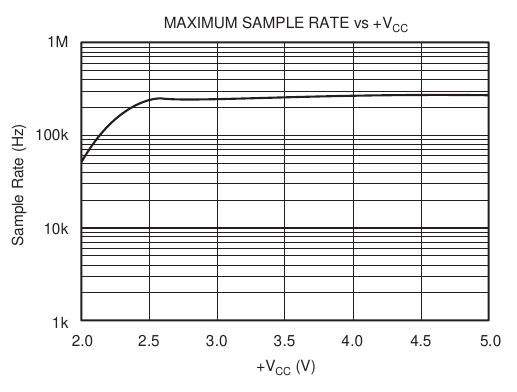
\includegraphics[width=\textwidth]{samplerate_vcc.png}
					\caption{Variation of the Sample Rate with $V_{CC}$}
					\label{fig:sample_vcc}
				\end{minipage}
				\begin{minipage}{.5\textwidth}
					\centering
					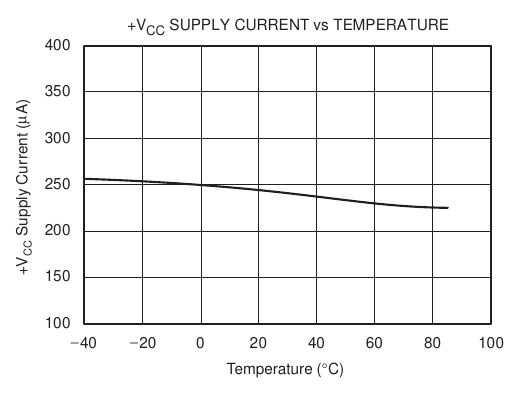
\includegraphics[width=\textwidth]{VCC_temp.png}
					\caption{Variation of $V_{CC}$ with the temperature}
					\label{fig:vcc_temp}
				\end{minipage}
			\end{figure}

			Finally, the temperature inside the chip is measured through a diode in the following way.
			The diode voltage $V_{BE}$ has a well-defined characteristic versus temperature, so the ambient temperature can be predicted in applications by knowing the +25°C value of the $V_{BE}$ voltage and then monitoring the delta of that voltage as the temperature changes.
		\newpage
		\subsubsection{Dual Antenna Wireless Module}
		\begin{figure}[htbp]
			\centering
			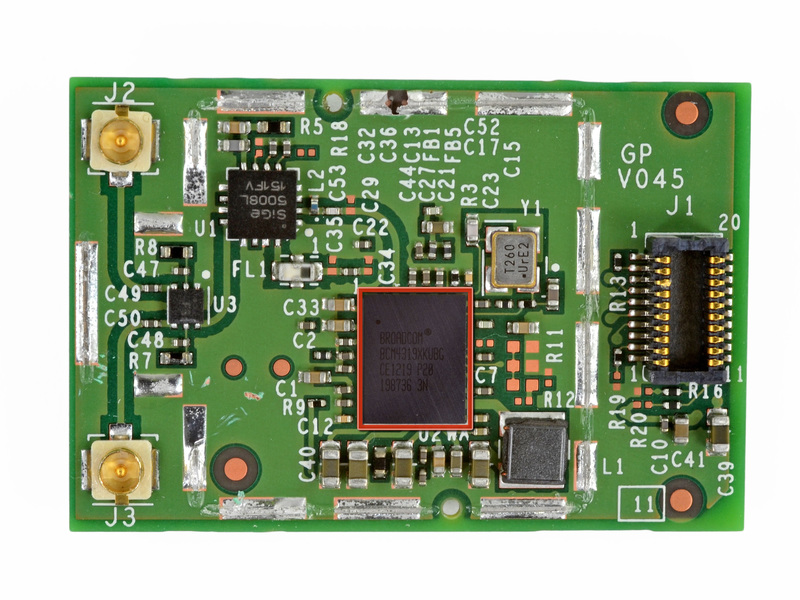
\includegraphics[width=.6\textwidth]{dual_antenna_wireless1.png}
			\caption{GamePad's wireless module}
			\label{fig:gamepad_wireless}
		\end{figure}
		Another module that can be extracted from the motherboard is the Dual Antenna Wireless Module, i.e. the module that allow to stream video and data between Wii U console and GamePad. It is shown in \autoref{fig:gamepad_wireless} and was mounted in place of the blue square in \autoref{fig:gamepad_motherboard}.

		This module is powered by a Broadcom BCM4319XKUBG (red square in \autoref{fig:gamepad_wireless}) and is explained in \cite{broadcom_wireless}.

		Its \gls{pmu} provides significant power savings by putting the BCM4319XKUBG into various power management states appropriate to the current environment and activities that are being performed. The \gls{pmu} enables and disables internal regulators, switches, and other blocks based on a computation of the required resources and the relationship between resources and the time needed to enable and disable them.

		Also the clock speed can be dynamically changed depending on the current requirements. Obviously, slower clock speeds are used wherever possible.

		Free different power states are defined:
		\begin{description}
			\item [Active Mode] All BCM4319XKUBG cores are powered up and fully functional. All required regulators are enabled and put in the most efficient mode.Clock speeds are dynamically adjusted by the \gls{pmu}.
			\item [Sleep Mode] All main clocks are shut down, only one clock is active and is used from the \gls{pmu} to wake up the chip. In Sleep mode, the primary power consumed is due to leakage current.
			\item	[Power-down mode] The BCM4319XKUBG is effectively powered off by shutting down all internal regulators. The chip is brought out of this mode by external logic re-enabling the internal regulators.

		\end{description}


\bibliographystyle{IEEEtran}
\bibliography{IEEEabrv,bibliography}

\end{document}
